\chapter{Results and Discussion}
I've tried three approaches to alleviate the compromise between low distortion and short scanning time in the potentiometric SECM.
The problem stems from the high \emph{RC} time-constant.
For a sufficiently small microelectrode, the resistance \emph{R} can be so high, that the time-constant is measured in seconds.
To arrive at the equilibrium potential of the measuring electrode, about 4$\times$\emph{RC} time must be allowed for the cell.
Such high equilibration period is not practical, since a high number of sampling points must be included in the image raster to achieve the desired high resolution, and the 4$\times$\emph{RC} equilibration period must be waited at every sampling point.
This means, for an image to be recorded with a step size of \emph{s} ($\upmu$m), image side length of \emph{L} ($\upmu$m), probe translation speed of \emph{v} ($\upmu$m/s), and an equilibration period of $t_e$ ($s$), it takes $t$ ($s$) time to complete the image, calculated with the following equation:

\begin{equation}
\label{eq:scantime}
	t = (L/s+1)^{2}\times(s/v + t_e)
\end{equation}

Using the example from the \emph{"Introduction"}, if \emph{R} = 1 G$\ohm$ and \emph{C} = 500 pF, then \emph{RC} = 0.5 s, and $t$ = 882 s, or about 16 min, since about $t_e = 4 \times RC$ is necessary to obtain the equilibrium electrode potential with good approximation.
To decrease the overall scanning time, there are a number of possibilities.
If \emph{L} or $t_e$ is decreased or \emph{v} or \emph{s} is increased, then $t$ is decreased.
But, if the scanned area or resolution cannot be decreased further, then manipulating \emph{L} and \emph{s} is not a viable option.
The parameters left are $t_e$ and $v$.
To decrease $t_e$ and maintain image quality, $RC$ must be decreased simultaneously.
This is the first approach I took, and is detailed in Section \ref{solid_result}.

In the second and third approaches I exploit the properties of the potentiometric response function:

\begin{equation}
\label{eq:rc}
        E_{cell}(t_{e}) = E_{cell}(\infty) + [E_{cell}(0) - E_{cell}(\infty)]e^{-t_{e}/RC}
\end{equation}
where $E_{cell}(t)$ is the cell potential difference at time $t_{e}$, $E_{cell}(\infty)$ is the equilibrium cell potential difference, $E_{cell}(0)$ is the cell potential difference prior to the change.
The more different $E_{cell}(0)$ and $E_{cell}(\infty)$ are, the more the difference between $E_{cell}(\infty)$ and $E_{cell}(t_{e})$ will be.
Distortion of an image can be measured as an average of the differences between $E_{cell}(\infty)$ and $E_{cell}(t_{e})$ at each point.
It can be lowered by carefully optimizing scanning patterns and algorithms, so that the probe passes through borders between regions of high and low concentrations as few times as possible.
This approach is detailed in Section \ref{patterns_result}.

In the third approach, I use the inverse of the potentiometric response function (Eq. \ref{eq:rc}) as deconvolution function.
Since the relationship between $t_e$, $E_{cell}(0)$, $E_{cell}(t_e)$ and $E_{cell}(\infty)$ is known, a prediction for the only unknown $E_{cell}(\infty)$ can be calculated.
This approach is detailed in Section \ref{dec_result}.

Additionally, to increase the probe translation speed $v$ and maximize the time available for cell potential equilibration ($t_e$), a custom SECM was built at our department, and used in the second and third approach.
Increasing $v$ has practical limitations, for a probe moving too fast between sampling points might stir the electrolyte.
Scanning speeds of commercially available SECM devices however, haven't reached this limit, and are in the range of several tens of micrometers per second at best, due to hardware or software restrictions.
With the custom built microscope, translation speeds up to 1000 $\upmu$m/s are possible.
	
	\newpage
	\section{Using solid-contact electrodes as potentiometric SECM probes}
	\label{solid_result}
Solid-contact electrodes have lower resistance, compared to their otherwise identical, liquid-contact counterparts.
This is due to two reasons.
The solid contact can be pushed down very close to the micropipette orifice, shortening the thickness of the highly resistive ion-selective membrane, and decreasing the overall electrode resistance.
The other reason is that instead of the internal solution -- which has high resistance --, a modified carbon fiber -- which has low resistance -- is used as the ion-to-electron transducer.
If $R$ is lower, $RC$ is lower, and the potentiometric cell becomes faster.


		\subsection{Electrode characterization and SECM images of a model system}
I constructed two Mg$^{2+}$-ion selective electrodes.
One used a liquid contact, and the other a solid contact.
Besides this difference, they were prepared identically.
Basic characterisation was performed for both.
Fig. \ref{fig:solid_liquid_calibration}A and \ref{fig:solid_liquid_calibration}B shows the calibration plots for the liquid, and solid contact electrode, respectively.
Sensitivities towards the primary ion (Mg$^{2+}$) were close to nernstian and very similar, 29.12 mV and 33.44 mV for the liquid and solid contact electrode, respectively.
The solid contact electrode had a slightly wider dynamic range, reaching below $10^{-5}$ M.
Selectivity coefficients, characterization of the potassium ion-selective electrode, and further characterization of the magnesium ion-selective electrode can be found in \cite{calugareanu2013ion}.

\begin{figure}[h]
\begin{tikzpicture}
\begin{axis}[xmin=-0.5, xmax=5.5, width=7cm,height=6cm,xlabel=pMg, ylabel={E vs. Ag/AgCl/3 M KCl, mV}, clip marker paths=true, xtick = {0,1,2,3,4,5}, ytick = {-20,0,20,40,60,80}, xminorticks=true, minor x tick num = 1]
\addplot [only marks, domain=0:5.5, mark=*] table {data/electrodes/liquid_calibration_plot.txt};
\addplot [domain=0:3, samples=500, line width=0.1mm] {86.8-x*29.12};
\node[anchor=north east] at (rel axis cs:0.98,0.98) {A};
\node[anchor=south west] at (rel axis cs:0,0) {\Delta S = 29.12 mV / pMg};
\node[anchor=south west] at (rel axis cs:0,0.1) {R$^2$ = 0.99833};
\end{axis}
\end{tikzpicture}
\hfill
\begin{tikzpicture}
\begin{axis}[xmin=-0.5, xmax=5.5, width=7cm,height=6cm,xlabel=pMg, ylabel={E vs. Ag/AgCl/3 M KCl, mV}, clip marker paths=true,xtick = {0,1,2,3,4,5}, ytick={-150,-120,-90,-60,-30,0}, xminorticks=true, minor x tick num = 1]
\addplot [only marks, domain=0:5.5, mark=*] table {data/electrodes/solid_calibration_plot.txt};
\addplot [domain=0:3.5, samples=500, line width=0.1mm] {-6.62-x*33.44};
\node[anchor=north east] at (rel axis cs:0.98,0.98) {B};
\node[anchor=south west] at (rel axis cs:0,0) {\Delta S = 33.44 mV / pMg};
\node[anchor=south west] at (rel axis cs:0,0.1) {R$^2$ = 0.99928};
\end{axis}
\end{tikzpicture}
\caption[Calibration plots for the Mg$^{2+}$ ISME.]{Calibration plots for the Mg$^{2+}$ ISME in 1 mM NaCl solutions containing varying amounts of MgCl$_2$ (pMg$^{2+} = -\log_{10} [$Mg$^{2+}]$).
(A) Liquid-contact, and (B) solid-contact.}
\label{fig:solid_liquid_calibration}
\end{figure}

Response characteristics were investigated by measuring the electrode resistance $R$, and the $\tau_{95}$ response time.
The two parameters are related: $1-e^{-3RC/RC} = 1-e^{-3} \approx 0.95$.
This means, that $3\times RC \approx \tau_{95}$, because in $3\times RC$, equilibrium electrode potential is reached by about 95\%.
Calculated from the voltage divider measurements (Fig. \ref{fig:solid_liquid_response_time}, Table \ref{table:comp}), electrode resistance was 4.8 $G\ohm$ and 0.56 $G\ohm$ for the liquid, and solid contact electrodes, respectively.
The measured $\tau_{95}$ parameters were 71.1 s, and 27.7 s, respectively (Fig. \ref{fig:solid_liquid_resistance}).
Based on these values, the solid contact electrode was expected to produce less distorted images with the same scanning parameters.

\begin{figure}
\centering
\begin{tikzpicture}
\begin{axis}	[
		only marks,
     		xmin=0,
		xmax=1400,
		ymin=-20,
		ymax=40,
		width=7cm,
		height=6cm,
		xlabel={time, s},
		ylabel={E vs. Ag/AgCl/3 M KCl, mV},
		/pgf/number format/.cd, use comma, 1000 sep={}
		]
		\addplot [mark=*, mark size=0.5] table {data/electrodes/liquid_response_time.txt};
		\node[anchor=north east] at (rel axis cs:0.98,0.98) {A};
\end{axis}
\end{tikzpicture}
\hfill
\begin{tikzpicture}
\begin{axis}	[
		only marks,
     		xmin=0,
		xmax=1400,
		ymin=-130,
		ymax=-70,
		width=7cm,
		height=6cm,
		xlabel={time, s},
		ylabel={E vs. Ag/AgCl/3 M KCl, mV},
		/pgf/number format/.cd, use comma, 1000 sep={}
		]
		\addplot [mark=*, mark size=0.5] table {data/electrodes/solid_response_time.txt};
		\node[anchor=north east] at (rel axis cs:0.98,0.98) {B};
\end{axis}
\end{tikzpicture}
\caption[Dynamic response curves obtained for response time measurements to changes in MgCl$_2$ concentrations.]{Dynamic response curves obtained for response time measurements to changes in MgCl$_2$ concentrations of 10$^{-1}$ M and 10$^{-2}$ M, in 10$^{-3}$ M NaCl.
(A) liquid-contact, and (B) solid-contact Mg$^{2+}$ ISME.}
\label{fig:solid_liquid_response_time}
\end{figure}

\begin{figure}
\centering
\begin{tikzpicture}
\begin{axis}	[
		only marks,
     		xmin=0,
		xmax=400,
		ymin=-70,
		ymax=20,
		width=7cm,
		height=6cm,
		xlabel={time, s},
		ylabel={E vs. Ag/AgCl/3 M KCl, mV},
		/pgf/number format/.cd, use comma, 1000 sep={}
		]
		\addplot [mark=*, mark size=0.5] table {data/electrodes/liquid_resistance.txt};
		\node[anchor=north east] at (rel axis cs:0.98,0.98) {A};
		\node[anchor=south west] at (axis cs:20,-60) {$\infty$};
		\node[anchor=south west] at (axis cs:90,-20) {0.5 G$\ohm$};
		\node[anchor=south west] at (axis cs:205,-23) {1 G$\ohm$};
		\node[anchor=south west] at (axis cs:320,-60) {$\infty$};
\end{axis}
\end{tikzpicture}
\hfill
\begin{tikzpicture}
\begin{axis}	[
		only marks,
     		xmin=0,
		xmax=400,
		ymin=-100,
		ymax=-20,
		width=7cm,
		height=6cm,
		xlabel={time, s},
		ylabel={E vs. Ag/AgCl/3 M KCl, mV},
		/pgf/number format/.cd, use comma, 1000 sep={}
		]
		\addplot [mark=*, mark size=0.5] table {data/electrodes/solid_resistance.txt};
		\node[anchor=north east] at (rel axis cs:0.98,0.98) {B};
		\node[anchor=south west] at (axis cs:20,-85) {$\infty$};
		\node[anchor=south west] at (axis cs:110,-55) {0.5 G$\ohm$};
		\node[anchor=south west] at (axis cs:230,-62) {1 G$\ohm$};
		\node[anchor=south west] at (axis cs:350,-85) {$\infty$};
\end{axis}
\end{tikzpicture}
\caption[Response of ISME to shorting resistors for the voltage divider method.]{Response of ISME to shorting resistors for the voltage divider method: (A) Liquid-contact, and (B) solid-contact.}
\label{fig:solid_liquid_resistance}
\end{figure}

To confirm it, a Mg$^{2+}$ ion diffusion source model system was created, and the plane 100 $\upmu$m above the pipette orifice was scanned with both electrodes.
Fig. \ref{fig:solid_liquid_pipette} shows the ISME images obtained using a liquid-contact (A), and a solid-contact (B), micropipette electrode.
Both 2D ISME maps were recorded at a scan rate of 12.5 $\upmu$m/s.
The same pipette holding the 0.1 M MgCl$_2$ agar solution was used in the measurements plotted in Figs. \ref{fig:solid_liquid_pipette}A and \ref{fig:solid_liquid_pipette}B.
Visual inspection of the two images clearly shows significant image distortion in the X-direction with the liquid-contact ISME due its slower response as expected based on its higher resistance.
It can also be observed in the image scanned with the solid-contact electrode, although to a much less extent.
The overlayed isoconcentric countour lines are more circular, and not as elongated in the X-direction as in the case of the image prepared with the convential electrode.
Another important feature to note in the images is the difference in the highest magnesium ion concentration observed with the two electrodes.
With the solid-contact microelectrode it's about $10^{-2.5}$ M.
On the other hand, with the conventional liquid-contact electrode, highest observed magnesium ion concentration is only about $10^{-3.4}$ M.
One possible reason for this is that the cell equipped with the liquid-contact electrode cannot keep up with the changes of the magnesium ion concentration at the micropipette orifice.
That is, it passes over the area with the highest concentration so quickly, that by the time the cell would reach the potential corresponding to that concentration, the probe is already at another location, with a lower concentration.
Potential starts dropping, while it approaches the new equilibrium potential.

\begin{figure}
\centering
% trim = top left bottom right
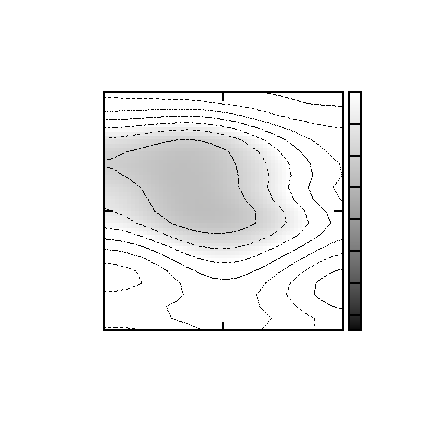
\includegraphics[trim = 10mm 30mm 0mm 20mm, clip, width=0.35\textwidth, angle=-90]{img/mg_pipette/liquid_Mg.eps} \includegraphics[trim = 10mm 30mm 0mm 20mm, clip, width=0.35\textwidth, angle=-90]{img/mg_pipette/solid_Mg.eps}
\caption[SECM images displaying the Mg$^{2+}$ ion concentrations 100 $\upmu$m above the tip of a centered pipette source.]{SECM images displaying the Mg$^{2+}$ ion concentrations 100 $\upmu$m above the tip of a centered pipette source.
(A) liquid-contact, and (B) solid-contact.
Scan rate: 12.5 $\upmu$m/s.}
\label{fig:solid_liquid_pipette}
\end{figure}


\begin{table}
                \caption[Resistance measurements for the two kinds of Mg$^{2+}$ ion-selective micropipette electrodes.]{Resistance measurements for the two kinds of Mg$^{2+}$ ion-selective micropipette electrodes conducted in 1 mM MgCl$_2$  1 mM NaCl solution.}
                \label{table:comp}
                \centering
                \begin{tabular}{r c c}
			& \multicolumn{2}{c}{ISME}\\
			\cline{2-3}
                        Parameter & Liquid-contact & Solid-contact \\
                        \hline
                        E$_{OCP}$ / mV & -49.5 & -75.5 \\
                        R / G$\ohm $ & 1 & 1 \\
                        U$_R$ / mV & -8.53 & -48.41 \\
                        R$_{ISME}$ / G$\ohm $ & 4.80 & 0.56 \\
                \end{tabular}
\end{table}

		\subsection{Applications}
			\subsubsection{Investigation of galvanic and homogeneous corrosion of magnesium}
In paper (II), we used the Mg$^{2+}$ ion-selective electrodes to image Mg$^{2+}$ ion concentration above the corroding samples and compared the results.
Based on the pipette source model target experiment and the resistivity measurements, it was expected that the cell equipped with the solid-contact electrode would yield less distorted images.
Fig. \ref{fig:solid_liquid_corrosion} shows the four scans.
Inspecting the images about the uncoupled magnesium (Fig. \ref{fig:solid_liquid_corrosion}A1-A2), it is clear that the image scanned with the liquid-contact electrode is more distorted.
The individual scanlines are blurred in the $X$ direction, just like in the previous experiment with the pipette source.
The same can be said about the images of the galvanically coupled magnesium.
The one scanned with the solid-contact electrode is less distorted.
Also, higher peak values can be observed, corresponding to magnesium dissolution.
These anodic spots are resolved much better by the solid-contact electrode.

\begin{figure}
\centering
% trim = top left bottom right
\includegraphics[trim = 10mm 40mm 0mm 40mm, clip, width=0.4\textwidth, angle=-90]{img/mg_metal/liquid_uncoupled.eps} \includegraphics[trim = 10mm 40mm 0mm 40mm, clip, width=0.4\textwidth, angle=-90]{img/mg_metal/solid_uncoupled.eps}

\includegraphics[trim = 10mm 40mm 0mm 40mm, clip, width=0.4\textwidth, angle=-90]{img/mg_metal/liquid_coupled.eps} \includegraphics[trim = 10mm 40mm 0mm 40mm, clip, width=0.4\textwidth, angle=-90]{img/mg_metal/solid_coupled.eps}
\caption[SECM scans above the magnesium sample with the solid- and liquid contact magnesium ion-selective micropipettes.]{SECM scans above the magnesium sample (A) uncoupled, and (B) galvanically coupled to the iron sample, while the cell was equipped with the conventional (1) liquid contact, and the new, (2) solid contact micropipette.
Scans were performed with the Sensolytics SECM, with impedance matching provided by the TL082 based voltage follower.
Reference electrode was Ag/AgCl/3M KCl.
Height of scan was 100 $\upmu$m, scanrate was 12.5 $\upmu$m/s.}
\label{fig:solid_liquid_corrosion}
\end{figure}

			\subsubsection{Estimation of corrosion current based on vertical SECM scans}
Mg$^{2+}$ ion concentration profiles above the Mg sample were recorded by SECM scans.
Vertical Mg$^{2+}$ ion concentration distribution was determined at different instants in time of the corrosion process, with, and without coupling the Mg/Al and Fe samples.
About ten times more Mg$^{2+}$ is being formed with coupling.
Mg$^{2+}$ concentration was increasing with time above the sample while coupled, on the other hand, it was decreasing after 10 minutes while not coupled (Fig. \ref{fig:retracting}A).
Based on the method of Scott and White \cite{scott1993iontophoretic}, using the Mg$^{2+}$ concentration profiles, Mg$^{2+}$ flow rate from the Mg piece was possible to estimate:

\begin{equation}
\label{eq:corrosion_current}
        \Omega = 4 D C_s a
\end{equation}

where $\Omega$ is the amount of Mg$^{2+}$ released from the disc shaped Mg/Al surface, $D$ is the diffusion coefficient of Mg$^{2+}$, $C_s$ is the surface concentration of Mg$^{2+}$ (at the height z = 0 $\upmu$m), a is the radius of the Mg/Al sample.
As the only unknown variable in the equation above, $\Omega$ could be calculated.
Substituting the value of D = 7.06$\times$10$^{-8}$ dm$^2 \cdot$s$^{-1}$ \cite{lide2001crc}, $C_s=3.29\times10^{-2}$ M, a = 0.0038 dm, the result is $\Omega$ = $3.53\times10^{-11}$ mol$\cdot$s$^{-1}$.

\begin{figure}
\centering
\begin{tikzpicture}
\begin{axis}	[legend style={draw=none},
		xmin=0,
		xmax=1,
		ymin=0,
		ymax=0.006,
		width=6cm,
		height=7cm,
		xlabel={height, mm},
		ylabel={[Mg$^{2+}$], mol$\cdot$dm$^{-3}$},
		clip marker paths=true]
\node[anchor=north west] at (rel axis cs:0.02,0.98) {A};
\addplot [mark=none, color=orange] table {data/approaching_scans/uncoupled/10min.txt};
\addplot [mark=none, color=yellow] table {data/approaching_scans/uncoupled/20min.txt};
\addplot [mark=none, color=green] table {data/approaching_scans/uncoupled/30min.txt};
\addplot [mark=none, color=cyan] table {data/approaching_scans/uncoupled/40min.txt};
\addplot [mark=none, color=blue] table {data/approaching_scans/uncoupled/50min.txt};
\addplot [mark=none, color=purple] table {data/approaching_scans/uncoupled/60min.txt};
\addlegendentry{10 min}
\addlegendentry{20 min}
\addlegendentry{30 min}
\addlegendentry{40 min}
\addlegendentry{50 min}
\addlegendentry{60 min}
\end{axis}
\end{tikzpicture}
\begin{tikzpicture}
\begin{axis}	[legend style={draw=none},
		xmin=0,
		xmax=1,
		ymin=0,
		ymax=0.1,
		width=6cm,
		height=7cm,
		xlabel={height, mm},
		%ylabel={[Mg$^{2+}$]},
		clip marker paths=true]
\node[anchor=north west] at (rel axis cs:0.02,0.98) {B};
\addplot [mark=none, color=orange] table {data/approaching_scans/coupled/10min.txt};
\addplot [mark=none, color=yellow] table {data/approaching_scans/coupled/20min.txt};
\addplot [mark=none, color=green] table {data/approaching_scans/coupled/30min.txt};
\addplot [mark=none, color=cyan] table {data/approaching_scans/coupled/40min.txt};
\addplot [mark=none, color=blue] table {data/approaching_scans/coupled/50min.txt};
\addplot [mark=none, color=purple] table {data/approaching_scans/coupled/60min.txt};
\addlegendentry{10 min}
\addlegendentry{20 min}
\addlegendentry{30 min}
\addlegendentry{40 min}
\addlegendentry{50 min}
\addlegendentry{60 min}
\end{axis}
\end{tikzpicture}

\begin{tikzpicture}
\begin{axis}	[legend style={draw=none},
		xmin=0,
		xmax=5,
		ymin=0,
		ymax=0.008,
		width=12cm,
		height=7cm,
		xlabel={lateral distance, mm},
		ylabel={[Mg$^{2+}$], mol$\cdot$dm$^{-3}$},
		clip marker paths=true]
\node[anchor=north west] at (rel axis cs:0.02,0.98) {C};
\addplot [mark=none, color=red] table {data/lateral_scans/5min.txt};
\addplot [mark=none, color=orange] table {data/lateral_scans/10min.txt};
\addplot [mark=none, color=yellow] table {data/lateral_scans/20min.txt};
\addplot [mark=none, color=green] table {data/lateral_scans/30min.txt};
\addplot [mark=none, color=cyan] table {data/lateral_scans/40min.txt};
\addplot [mark=none, color=blue] table {data/lateral_scans/50min.txt};
\addplot [mark=none, color=purple] table {data/lateral_scans/60min.txt};
\addlegendentry{5 min}
\addlegendentry{10 min}
\addlegendentry{20 min}
\addlegendentry{30 min}
\addlegendentry{40 min}
\addlegendentry{50 min}
\addlegendentry{60 min}
\end{axis}
\end{tikzpicture}
\caption[Retracting and lateral SECM linescans above the AZ63 sample initiated at different instances in time.]{Retracting and lateral SECM linescans above the AZ63 magnesium-aluminium-zinc alloy sample initiated at different instances in time.
Scan rate: 10 $\upmu$m/s.}
\label{fig:retracting}
\end{figure}

Corrosion current between the Mg/Al sample and four Fe samples with different diameters was also measured directly.
As expected, current gets higher with increasing diameter.
Corrosion current was 8.87 $\upmu$A, 15.83 $\upmu$A, 16.72 $\upmu$A, 24.4 $\upmu$A with Fe sample diameters of 0.59 mm, 0.76 mm, 1.2 mm, 2.3 mm, respectively (Fig. \ref{fig:corrosion_current_measurements}).
Using Faraday's law of electrolysis, this means, that $8.20\times10^{-11}$ mol Mg$^{2+}$ is being dissolved in every second from the Mg/Al sample ($\Omega_{0.76 \textrm{mm}} = 8.20\times10^{-11} mol/s$).
This result is in fairly good agreement with the SECM measurement ($\Omega = 3.53\times10^{-11}$ mol/s).
Ion flow rates from Mg/Al samples coupled with Fe samples of different diameters are proportional with the surface area of the sample; $\Omega_{0.59mm} = 4.60\times10^{-11} mol/s, \Omega_{1.2mm} = 4.66\times10^{-11} mol/s, \Omega_{2.3mm} = 1.26\times10^{-10} mol/s$.

\begin{figure}
\centering
% trim = top left bottom right
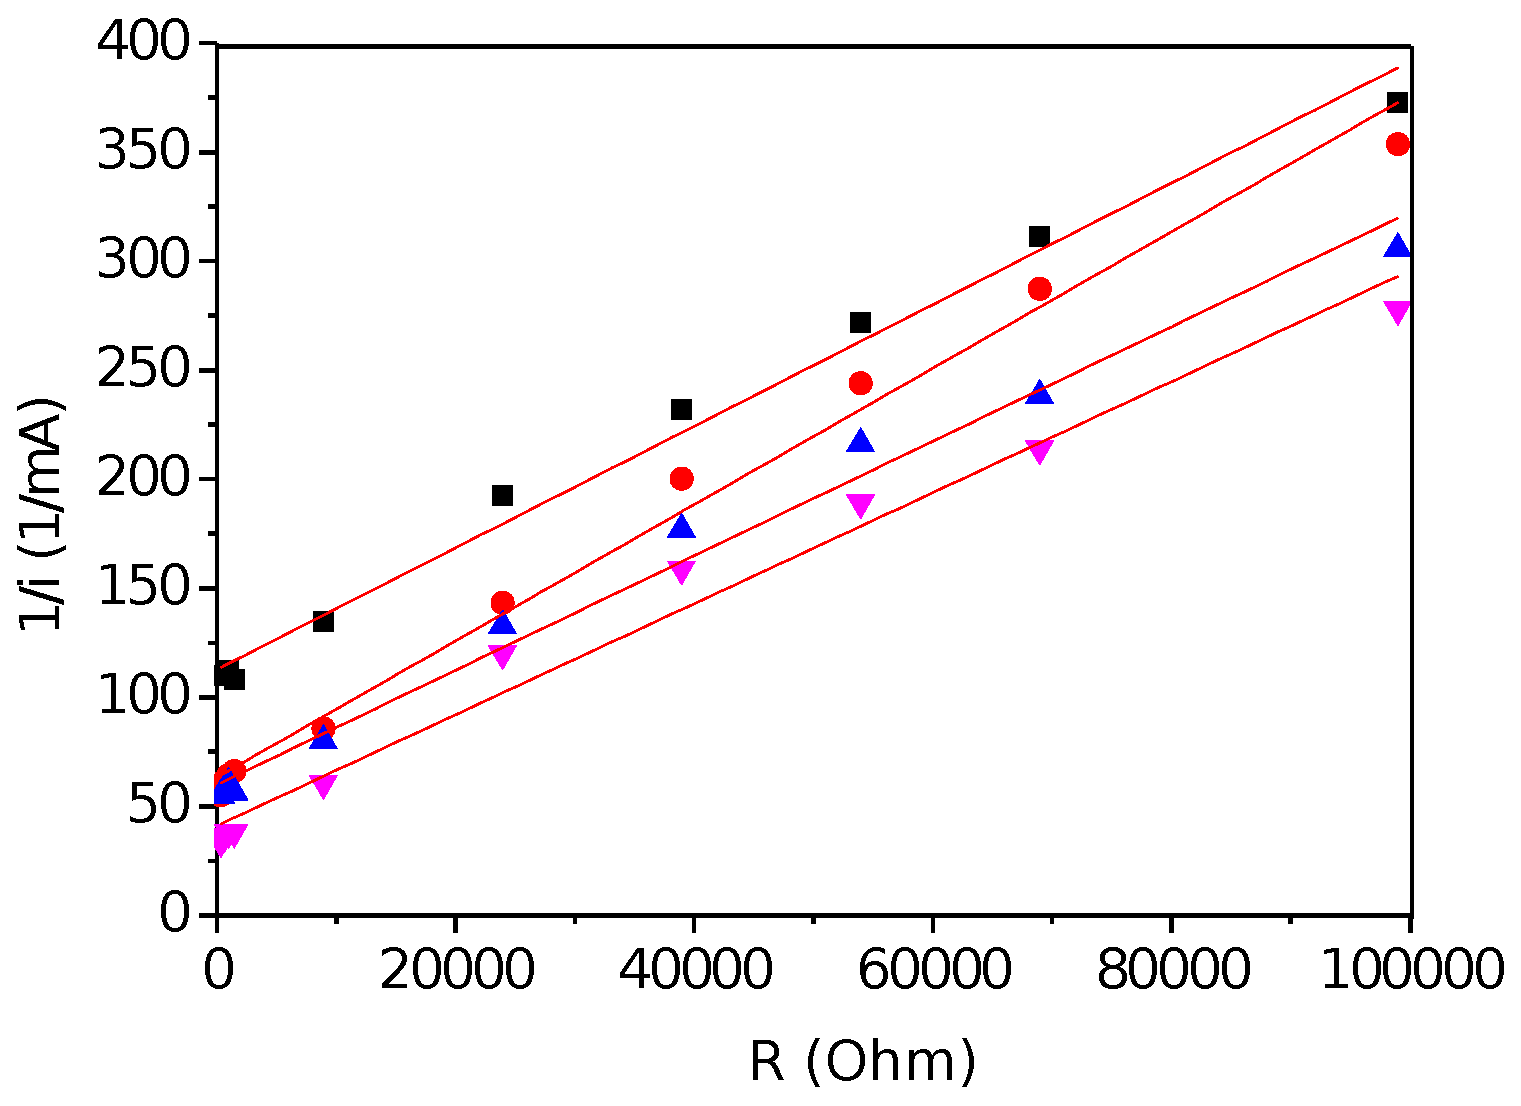
\includegraphics[width=0.6\textwidth]{img/corrosion_current_measurements.eps} 
\caption[1/i plots used for the determination of corrosion current between the AZ63 magnesium-aluminium-zinc alloy and various iron samples of different diameters.]{1/i plots used for the determination of corrosion current between the AZ63 magnesium-aluminium-zinc alloy and various iron samples of different diameters.
Diameter of the iron cathodes; black rectangle: d = 0.59 mm, red circle: d = 0.76 mm, blue triangle d = 1.2 mm, purple upside-down triangle: d = 2.3 mm.}
\label{fig:corrosion_current_measurements}
\end{figure}

	\newpage
	\section{Optimization of scanning algorithms}
	\label{patterns_result}
		\subsection{SECM simulations}
To obtain high quality images in scanning probe microscopy, a certain amount of scanning time is required, depending on the number of sampling points, and the scanning speed.
Usually, there is a compromise between scanning speed and image quality.
This is most critical in the potentiometric scanning electrochemical microscopy, which is severely limited by the relatively long response time of the ultramicro-electrode probes.
That is, scanning speed can be increased only at the expense of image quality.

In a great majority of the SECM studies, the subjects are circularly symmetric systems.
In this section, I present a method to increase SECM imaging speed of such systems, while improving image quality at the same time.
It is achieved by using new, polar coordinate-based scanning patterns, exploiting the symmetry of the studied system, and using imaging time more economically.
This technique significantly improves the imaging of circularly symmetric targets.

Numerical simulations and SECM scans using the traditional, and the new scanning algorithms have
been performed. The resulting images have been compared with the expected, ideal image.

First, SECM scanning simulations were performed and the resulting images were compared (Figure \ref{fig:simulations}).
It was expected that the new, polar coordinate-based scanning algorithms would yield less distorted images than the traditional, raster-based algorithms.
Not only the two new algorithms finish faster, but result images with lower distortion (Table \ref{table:comp}).
Mean squared error is $9.63\times 10^{-3}$ and $2.95\times 10^{-3}$ for the images scanned with the web and the arc algorithms, respectively.
In comparison, mean squared error for the images scanned with traditional meander, fast-comb, and comb algorithms are $2.75\times 10^{-2}$, $2.07\times 10^{-2}$, and $2.75\times 10^{-2}$, respectively.

		\subsection{Experimental SECM images}
Next, the experimental SECM scans were performed, with the same scanning algorithms as the simulations were.
The results (Figure \ref{fig:measurements}) confirmed our presumption, that using the two new algorithms, images have less distortion, with higher similarity to the expected image.

Considering scanning time also, which are 440, 520, and 881 seconds for the meander, fast-comb, and comb algorithms, and 109, and 340 seconds for the web, and arc patterns respectively, it can be said, that the new scanning algorithms proposed in this paper shorten scanning time, and significantly improve imaging quality of circularly symmetric systems.
There are two additional advantageous properties of the new algorithms.
First, data is gathered in order of decreasing relevance, from closest to the target, to farthest from the target, without the corners of the rectangular raster patterns, which are of less importance, because of the larger distance from the target.
Second, with the new algorithms, there is only positive imaging distortion (Figure \ref{fig:patterns}I, J).
The observed potential, for a perfect hemispherical concentration distribution, in theory, cannot be lower above the center than the maximum value.
It also cannot be higher, since the probe starts scanning in the center, where $E_{cell}(t) \approx E_{cell}(\infty)$ (Equation \ref{eq:rc}).
But positive distorion can occur as the probe leaves the close vicinity of the target, advancing towards coordinates with lower concentration.
This has an importance when accurate quantitative information is required about the concentration distribution above the target, such as in estimating fluxes by fitting simulation to measured images \cite{gyurcsanyi2004chemical, kiss2011air}.

\newpage
\begin{figure}[H]
\centering
% trim = top left bottom right
\includegraphics[trim = 20mm 30mm 0mm 20mm, clip, width=0.25\textwidth, angle=-90]{img/sim/meander_sim.eps} \includegraphics[trim = 20mm 30mm 0mm 20mm, clip, width=0.25\textwidth, angle=-90]{img/sim/meander_delta.eps}

\includegraphics[trim = 20mm 30mm 0mm 20mm, clip, width=0.25\textwidth, angle=-90]{img/sim/fastcomb_sim.eps} \includegraphics[trim = 20mm 30mm 0mm 20mm, clip, width=0.25\textwidth, angle=-90]{img/sim/fastcomb_delta.eps}

\includegraphics[trim = 20mm 30mm 0mm 20mm, clip, width=0.25\textwidth, angle=-90]{img/sim/comb_sim.eps} \includegraphics[trim = 20mm 30mm 0mm 20mm, clip, width=0.25\textwidth, angle=-90]{img/sim/comb_delta.eps}

\includegraphics[trim = 20mm 30mm 0mm 20mm, clip, width=0.25\textwidth, angle=-90]{img/sim/web_sim.eps} \includegraphics[trim = 20mm 30mm 0mm 20mm, clip, width=0.25\textwidth, angle=-90]{img/sim/web_delta.eps}

\includegraphics[trim = 20mm 30mm 0mm 20mm, clip, width=0.25\textwidth, angle=-90]{img/sim/arc_sim.eps} \includegraphics[trim = 20mm 30mm 0mm 20mm, clip, width=0.25\textwidth, angle=-90]{img/sim/arc_delta.eps}

\caption[Simulated SECM scans 100 $\upmu$m above the disc source and deviation from the original images.]{(A-E) Simulated SECM scans 100 $\upmu$m above the disc source with the meander, fast comb, comb, web, and the arc scanning algorithms, respectively.
All images were normalized to the maximum concentration of the expected image (c$_{max}$).
(F-J) Deviation from the expected concentration image using the meander, fast comb, comb, web, and the arc scanning algorithms, respectively.
,,$C$'' is the input (expected concentration profile), ,,$c$'' is the output (observed concentration profile) matrix for the scan simulation.}
\label{fig:simulations}
\end{figure}

\newpage
\begin{figure}[H]
\centering
% trim = top left bottom right 
\includegraphics[trim = 10mm 30mm 0mm 10mm, clip, width=0.25\textwidth, angle=-90]{img/polar/meander.eps} \includegraphics[trim = 10mm 30mm 0mm 10mm, clip, width=0.25\textwidth, angle=-90]{img/polar/fastcomb.eps}

\includegraphics[trim = 10mm 30mm 0mm 10mm, clip, width=0.25\textwidth, angle=-90]{img/polar/comb.eps} \includegraphics[trim = 10mm 30mm 0mm 10mm, clip, width=0.25\textwidth, angle=-90]{img/polar/web.eps}

\includegraphics[trim = 10mm 30mm 0mm 10mm, clip, width=0.25\textwidth, angle=-90]{img/polar/arc.eps}

\caption[Experimental SECM scans 100 $\upmu$m above the disc source.]{Experimental SECM scans 100 $\upmu$m above the disc source with the (A) meander, (B) fast comb, (C) comb, (D) web, and (E) the arc scanning algorithms.
Measuring electrode was a pH-sensitive antimony micro-electrode.
Potential was measured against an Ag/AgCl/3M KCl reference electrode.}
\label{fig:measurements}
\end{figure}

\begin{table}
                \caption{Comparison of the scanning algorithms.}
                \label{table:comp}
                \centering
                \begin{tabular}{r c c c}
                        Algorithm & Number of sampling points & Total scan time (s) & Mean squared error \\
                        \hline
                        Meander & 441 & 440 & $2.75\times 10^{-2}$ \\
                        Fast comb & 441 & 520  & $2.07\times 10^{-2}$ \\
                        Comb & 441 & 881 & $2.75\times 10^{-2}$ \\
                        Web & 110 & 109 & $9.63\times 10^{-3}$ \\
			Arc & 341 & 340 & $2.95\times 10^{-3}$ \\
                \end{tabular}
\end{table}

	\newpage
	\section{Signal processing in potentiometric SECM}
	\label{dec_result}

		\subsection{Deconvolution of measurements performed with metal/metal-oxide microelectrodes}
In order to image rapidly changing systems with the Scanning Electrochemical Microscope, high scan rate must be used, otherwise by the time the scan is completed, major changes in the studied system would have occured.
But if the scan rate is too high, there is not enough time for the detector to reach equilibrium before the signal is recorded at a given data acquisition point, and the image will be distorted.
This is a problem especially in potentiometric SECM, where the long response time of the potentiometric cell using ultramicro electrode probes imposes a limit on the maximum scan rate.
In this section I demonstrate that high scan rates combined with signal processing can be used in potentiometric SECM to keep scan time to a minimum, and still obtain high quality results by deconvoluting the raw, distorted image.
Model systems were studied with high scan rate, then the images were deconvoluted using the inverse of the potentiometric response function to calculate the equilibrium value for each data acquisition point from the respective observed values.

Deconvolution of measurements obtained with the metal/metal-oxide electrodes (antimony/antimony-oxide, and tungsten/tungsten-oxide) are attempted.
First, a simple step response, then 1D linescans, and finally 2D raster images were deconvoluted, using four different electrodes; pH sensing microelectrodes made from antimony and tungsten, and ion selective microelectrodes for magnesium and potassium ions.
This method has been already proposed in 1981 to determine the response time of potentiometric cells, based on the initial portion of the response curve, since it holds the same information.
However, the authors of the paper about that method didn't go any further with their proposition.
As Lindner and his coauthors write in \cite{lindner1984definition}:

\begin{quote}
\vspace{0.5cm}
\emph{,,This new definition [of response time] has several advantages in contrast to the earlier propositions and accepted definitions: it does not require the knowledge of the equilibrium potential value ($E_{\infty}$); it holds the same sort of information as the time constant of a theoretical equation; it can be used in the case of response time curves consisting of different sections, e.g., even for rapid kinetic studies when $t \approx 0$ (6), and in practice it helps the analysts in determining when potential readings are to be taken.
Accordingly to eliminate subjective errors in readings, one can regard the potential value corresponding to a limiting slope (dE/dt) as the steady-state or equilibrium value.
This idea is realized in some pH meters produced by Radelkis (Hungary) in which a so-called slope controller is built in (16).
\footnote{(6) refers to \cite{lindner1982response} and (16) refers to \cite{havas1981}}''}
\vspace{0.5cm}
\end{quote}


			\subsubsection{Minimal working example: deconvolution of a step response}
The ,,minimal working example'' method, originally used in programming, is a way of tracking down problems, and finding the cause of certain behaviour.
The most important feature of a minimal working example is that it is as simple as possible, such that it is just sufficient to demonstrate the problem, but without any additional complexity which would make resolution harder.
In this case, the minimal working example is a simple step function: the activity of the primary ion is changed suddenly, while the response of the potentiometric cell is recorded.
The input of the system is a step function, the output is the recorded signal, an exponential decay function.
If there is no additional distortion, and the transfer function is simply Eq. \ref{eq:rc2}, the square step should be restored. 

To measure the time-constant of the potentiometric cell employing the antimony microelectrode, the transient response curve was recorded while the pH = 4 buffer solution was changed to pH = 6.
Then, Eq. \ref{eq:rc} was fitted on the curve (Fig. \ref{fig:transient}).
Based on the fit, time constant of the cell is $\tau = 3.76$ s, and $e^{-0.5 \; s/3.76 \; s} = 0.8755$, which means, only 12\% of the total change occurs in 0.5 s ($1 - 0.8755 = 0.1245$). 

\begin{figure}
\centering
\begin{tikzpicture}
\begin{axis}[ymin=-290, ymax=-170, xmin=-30, xmax=100, xlabel={time, s}, ylabel={E vs. Ag/AgCl/3 M KCl, mV}, clip marker paths=true, width=12cm, height=8cm, legend style={draw=none}, legend cell align=left]
\addplot [only marks, domain=-30:100, color=gray, mark=*] table {data/transient_aligned.txt};
\addplot [domain=0:100, samples=500, color=red, line width=0.4mm] {-280+(280-183)*exp(-x/3.76)};
%\addplot [domain=0:100, samples=500, color=green, line width=0.4mm] {-280+(280-183)*(exp(-x/9) + exp(-x/0.5577))/2};
%\addplot [domain=0:100, samples=500, color=blue, line width=0.4mm] {-280+(280-183)*(1/(1+sqrt(x)))};
%\addplot [domain=0:100, samples=500, color=cyan, line width=0.4mm] {-280+(280-183)*(1/(1+sqrt(0.000000000001*x)))*exp(-x/0.5577)};

%\addplot [domain=0:100, samples=500, color=green, line width=0.4mm] {-280+(280-183)*exp(-x/9)};
%\node[red, above right] at (axis cs:5,-200) {$y = - 280 + 97 \times e^{-x/3.76}$};
%\node[blue, above right] at (axis cs:5,-220) {$y = - 280 + 97 \times (e^{-x/9} + e^{-x/0.6})/2$};
\node[black, above left] at (axis cs:0,-290) {pH 4};
\node[black, above right] at (axis cs:0,-290) {pH 6};
%\addplot +[mark=none] coordinates {(0, -300)-.- (0, -100)};
\draw [dashed, black] (axis cs:0,-300) -- (axis cs:0,-100);
\addlegendentry{raw recording}
\addlegendentry{$E = - 280 + 97 e^{-t/3.76}$}
%\addlegendentry{$E = - 280 + 97 (e^{-t/9} + e^{-t/0.5577})/2$}
\end{axis}
\end{tikzpicture}
\caption[Transient response of the antimony microelectrode to analyte activity step.]{Transient response of the antimony microelectrode to analyte activity step.
The measuring and reference electrodes were dipped into buffer solutions with pH = 4 before the measurements started, and pH = 6 at t = 0 s, respectively.
Eq. \ref{eq:rc} was fitted (red line) on the measurement (gray marks) from the pH step to the end of the curve when potential reaches equilibrium in the pH = 6 buffer.}
\label{fig:transient}
\end{figure}


\begin{figure}
\centering
\begin{tikzpicture}
\begin{axis}	[legend style={draw=none},
		xmin=30,
		xmax=100,
		ymin=-350,
		ymax=-100,
		width=12cm,
		height=10cm,
		xlabel={time, s},
		ylabel={E vs. Ag/AgCl/3 M KCl, mV},
		clip marker paths=true]
\addplot [only marks, domain=30:100, color=red, mark=*] table {data/step_response/original.txt};
\addplot [only marks, domain=30:100, color=orange, mark=*] table {data/step_response/deconvoluted070.txt};
\addplot [only marks, domain=30:100, color=yellow, mark=*] table {data/step_response/deconvoluted075.txt};
\addplot [only marks, domain=30:100, color=green, mark=*] table {data/step_response/deconvoluted080.txt};
\addplot [only marks, domain=30:100, color=cyan, mark=*] table {data/step_response/deconvoluted085.txt};
\addplot [only marks, domain=30:100, color=blue, mark=*] table {data/step_response/deconvoluted090.txt};
\addplot [only marks, domain=30:100, color=purple, mark=*] table {data/step_response/deconvoluted095.txt};
%\addplot [only marks, domain=30:100, color=black, mark=*, x filter/.code={\pgfmathparse{\pgfmathresult+50}}] table {data/step_response/absolute_deconvoluted.txt};
\addlegendentry{raw recording}
\addlegendentry{RC = 1.40 s}
\addlegendentry{RC = 1.74 s}
\addlegendentry{RC = 2.24 s}
\addlegendentry{RC = 3.76 s}
\addlegendentry{RC = 4.75 s}
\addlegendentry{RC = 9.75 s}
%\addlegendentry{absolute}
\end{axis}
\end{tikzpicture}
\caption[]{Transient response of the antimony microelectrode to analyte activity step (red), and decovolutions performed with different assumed $RC$ time-constants (orange-purple).
The measured time-constant was $\tau = 3.76$ s (cyan).
The measuring and reference electrodes were dipped into buffer solutions with pH = 4 and pH = 6 respectively.}
\label{fig:deconvoluted_transient}
\end{figure}

The deconvolution of the very same recording was performed with several different time-constants, including that obtained from the response curve.
Fig. \ref{fig:deconvoluted_transient} shows the results of those deconvolutions.
As expected, the recording becomes most similar to the step function when the measured $RC$ time-constant is used.
When a higher value was substituted into Eq. \ref{eq:rc2}, the recorded potential was underestimated, and the deconvolution recovered more than necessary.
If a lower value was used, the cell was assumed to be faster than it actually was, and the deconvoluted potential values did not reach the equilibrium values.
To see the effect of using a time constant other than the one that was obtained from the fit, statistics was performed on the deconvoluted data.
Mean squared error was calculated by first taking the difference between the input function and the deconvoluted function at every time instance.
Then the square of those differences was averaged.
The input function was defined as 

\begin{equation}
E_{cell}(t) =
\left\{
	\begin{array}{ll}
		-183.18 \; \textrm{mV,} & \mbox{if } t < 50 \; \textrm{s} \\
		-280.20 \; \textrm{mV,} & \mbox{if } t \geq  50 \; \textrm{s}
	\end{array}
\right.
\label{eq:piecewise}
\end{equation}

The values for initial ($E_{cell}(0) = -183.18$ mV) and equilibrium ($E_{cell}(\infty) = -280.20$ mV) potentials were obtained by averaging certain portions of the recorded signal: the average from 0 to 49 s is $-183.18$ mV, and the average from 60 to 80 s is $-280.20$ mV.
\ref{eq:piecewise} should be obtained experimentally if the potentiometric cell was infinitely fast, and $RC$ would be 0.

\begin{table}
                \caption{Comparison of the deconvoluted time-potential recordings with different assumed time-consants, including the measured value (highlighted in bold).}
                \label{table:rc}
                \centering
                \begin{tabular}{r c c c}
                        $e^{-0.5/RC}$ & $RC (s)$ & Mean squared error \\
                        \hline
                        raw recording (0) & raw recording (0) & 53.43 \\
                        0.7 & 1.4 & 22.03  \\
                        0.75 & 1.74 & 15.88  \\
                        0.8 & 2.24 & 9.01 \\
			\textbf{0.8755} & \textbf{3.76} & \textbf{3.83} \\
			0.9 & 4.75 & 16.99 \\
			0.95 & 9.75 & 781.94 \\
                \end{tabular}
\end{table}

Table \ref{table:rc} shows the results of the statistical evaluation.
Mean squared error rapidly increases when instead of the measured time constant, smaller or larger values were used in the deconvolution.

\subsubsection{Investigation of possible surface processes}

There are two interesting properties of the fit in Fig. \ref{fig:transient}. to be noted.
First, the fitted curve is slightly different than the recorded response.
The initial part of the measurement seems to be changing faster than it is expected from an RC circuit with a time-constant of 3.76 s, while the second part (from around 7 s) has a lower rate of change compared to the model.
This means, that the transfer function is more complicated than Eq. \ref{eq:rc2}, and the process cannot be properly described by simple potentiometric step response function.
The effect of this behaviour can be observed in the first few data points of the deconvoluted measurement: there is a small overshoot compared to the equilibrium potential, even in the one that was deconvoluted with the measured $RC$.
It was observed in all of the measurements, and the error was certainly carried through to all of the deconvoluted images, when the original measurement was performed with the antimony microelectrode. 

The second discrepancy is that the $RC$ determined in the previous section implies a very high resistance (G$\ohm$ range).
It is possible to estimate the resistance of the antimony microelectrode from the specific resistance and the geometry of the antimony wire.
Diameter, as mentioned in the chapter \emph{,,Materials and Methods''}, was 30 $\upmu$m, length of the antimony wire was around 5 cm.
Specific resistance of antimony is 417 n$\ohm$m (at 20 $\celsius$) \cite{lide2001crc}.
Then, resistance could be calculated as $R$ = 417 n$\ohm$m $\times$ 0.05 m / ((15 $\upmu$m)$^2 \times \pi) = 29.50\; \ohm$.
It must be noted however, that the measured resistance is a property of the whole cell, not just the microelectrode.
Resistance of the reference electrode and the solution are included.
Nevertheless, the difference between the estimated and the measured values is still too high.
The very significant deviation from the expected value just calculated can be explained by a discontinuity defect in the antimony electrode, although it is unlikely, since all of the antimony electrodes appeared to have such a high resistance.

To verify that there was no discontinuity in the antimony microelectrodes, their resistance was measured directly by attaching one probe of a high precision multimeter to the microelectrode, while submersing the other probe and the tip of the microelectrode into a beaker containing mercury.
Several electrodes has been tested this way, and their resistance never exceeded 20 $\ohm$.
The typical value was around 12 $\ohm$, comparable to what was calculated from the electrode geometry and specific resistance of antimony.

Then, resistance of the whole cell was measured with the voltage divider method.
Open circuit potential was $-219.9$ mV, while potential difference while the terminals were shorted through a 200 k$\ohm$ precision resistor was $-105.0$ mV.
Resistance based on this result is 218.86 k$\ohm$, which is the sum of the resistances of the microelectrode, the reference electrode, and the solution.
This resistance is still not large enough to explain an RC time constant of 3.76 s, since then the capacitance should be 17.2 $\upmu$F, but it was in fact 11.15 nF (see section \ref{capacitance}.).

Another way it could be explained is that there is a strongly adhered laminar layer (Prandtl-layer) on the surface of the electrode, and the exchange of this layer in a new solution is the slowest process as it is discussed by Lindner et al. in \cite{lindner1976response}.
To test this hypothesis, step response measurements were carried out in unstirred and stirred buffers. The measuring electrode in this case was a large ($d$ = 1 mm) antimony disc electrode, with a silver/silver-chloride quasi-reference electrode separated by 1 mm of epoxy resin. Because the antimony surface is much larger than in the case of a microelectrode, a more delayed response can be expected in the unstirred case, if there is indeed an adhered layer on the surface. By stirring the buffers when they are exchanged, the time constant should be the much lower RC time constant, with R = 218.86 $\ohm$. 

\begin{figure}
\centering
\begin{tikzpicture}
\begin{axis}[ymin=-370, ymax=-200, xmin=0, xmax=750, xlabel={time, s}, ylabel={E vs. Ag/AgCl/3 M KCl, mV}, clip marker paths=true, width=12cm, height=6cm, legend style={draw=none}, legend cell align=left]
\addplot [domain=0:750, color=red, mark=*] table {data/stirring/stirring.txt};
\node[black, above left] at (axis cs:450,-370) {stirring off};
\node[black, above right] at (axis cs:450,-370) {stirring on};
\draw [dashed, black] (axis cs:450,-370) -- (axis cs:450,-200);
%\node[black, above left] at (axis cs:210,-330) {pH = 7};
%\node[black, above left] at (axis cs:210,-230) {pH = 4};
\end{axis}
\end{tikzpicture}
\caption[The effect of stirring on the antimony microelectrode.]{The effect of stirring on the antimony microelectrode.
The buffer solutions were quickly changed back and forth between pH = 4 ($E \approx -240$ mV) and pH = 7 ($E \approx -340$ mV).
Stirring was turned on at $t$ = 450 s.
To realize a quick change of the buffer solution without interrupting the potentiometric circuit, the \emph{,,hanging drop method''} was used. For this experiment, the Arduino-based home-made DAQ was used.}
\label{fig:stirring}
\end{figure}

Indeed, the response is much more delayed than in the case of a microelectrode, which can be observed in the response curves.
The cell employing the microelectrode had an almost 100\% response in about 1 minute (Fig. \ref{fig:transient}), while with the macroelectrode $\sim$100\% response was reached in about 200 s (first part of the curve in Fig. \ref{fig:stirring}.).
After stirring was turned on, the cell responded almost instantaneously (Fig. \ref{fig:stirring}) to analyte acivity step (that is depicted by the second part of the curve, after 450 s).
Unfortunately, the magnetic stirrer introduced so much noise, that the time constant couldn't be determined from this measurement.
In another experiment, a filter was applied to decrease noise, but, as an RC filter, it added a time constant of its own to the measurement, and thus it could not be evaluated.

Despite this discrepancy, with deconvolution, a sharp step function could be obtained from the potential-time measurement, which was very similar to the step function caused by the sudden change in activity of the hydrogen ions.
This means, that whatever the cause of the difference between the calculated and estimated resistance is, it distorts the measurement in a very similar way to the $RC$ distortion. Based on the stirring experiments, this is most likely a surface process. Perharps the antimony-oxide on the surface of the antimony microelectrode is porous, and it hinders diffusion. This behaviour wasn't studied any further in this thesis. Since the recorded step response includes every parameter affecting the delay, the fitted function already accounts for this behaviour. The deconvolution function is certainly not complete and far from perfect. However, all deconvolution in this thesis was perfomed in a stepwise manner; by only using one $x-y$ pair from Eq. \ref{eq:rc2}. $X$ coordinate was most often 0.5 s, the time that elapses between two consecutive measurements. That part of the deconvolution function seems to describe the system very well.

			\subsubsection{Linescans with the antimony microelectrode}

Going further, deconvolution of the simplest SECM experiment, the deconvolution of linescans was attemped.
The potentiometric cell included the same measuring and reference electrodes as in the previous sections.
A model system was built to perform the linescan on.
In the system, a hemispherical pH gradient was created.
The measured time constant ($\tau = 3.76$ s), implies a significant amount of imaging distortion if the equilibration period is only $t_e = 0.5$ s.
As mentioned in the previous section, during 0.5 s, only about 12\% of the total change occurs, and the measured difference between the recorded signal at two consecutive data aquisition points is significantly less than the difference between the equilibrium potentials.
Since a single linescan can be completed very quickly, for reference a linescan was performed with $t_e = 5$ s.
With this equilibration interval, the recorded potential at each point can be regarded equilibrium potential, and the linescan can be used as reference for the deconvoluted linescans performed with shorter $t_e$.
Fig. \ref{fig:lines_pH}A shows the raw linescans 100 $\upmu$m above the graphite anode.
Indeed, with $t_e = 0.5$ s, a significant amount of distortion can be observed.
When $t_e$ was increased to 1 s, the distortion decreased.
After deconvolution however, all of the linescans became similar to the equilibrium linescans, regarding both their peak value, and shape (Fig. \ref{fig:lines_pH}B).


\begin{figure}
\centering
\begin{tikzpicture}
\begin{axis}	[xmin=-1000,
		xmax=1000,
		width=6cm,
		height=6cm,
		xlabel=x / $\upmu$m,
		ylabel=E / V,
		/pgf/number format/.cd, use comma, 1000 sep={}]
\addplot [color=green] table {data/pH_linescans/500ms.txt};
\addplot [color=blue] table {data/pH_linescans/1000ms.txt};
\addplot [color=red] table {data/pH_linescans/5000ms.txt};
\end{axis}
\end{tikzpicture}
\begin{tikzpicture}
\begin{axis}	[xmin=-1000,
		xmax=1000,
		width=6cm,
		height=6cm,
		xlabel=x / $\upmu$m,
		ylabel=E / V,
		/pgf/number format/.cd, use comma, 1000 sep={}]
\addplot [color=green] table {data/pH_linescans/500ms_deconvoluted.txt};
\addplot [color=blue] table {data/pH_linescans/1000ms_deconvoluted.txt};
\addplot [color=red] table {data/pH_linescans/5000ms_deconvoluted.txt};
\end{axis}
\end{tikzpicture}
\caption[Raw and deconvoluted SECM linescans with the antimony microelectrode.]{(A) Raw, and, (B) deconvoluted SECM linescans above the center of the target, at h = 100 mm height, using three different equilibration periods: 0.5 s, (green), 1 s, (blue), and 5 s, (red).}
\label{fig:lines_pH}
\end{figure}

	\subsubsection{2D scans with the antimony microelectrode}
\begin{figure}
\centering
% trim = top left bottom right
\includegraphics[trim = 10mm 30mm 0mm 10mm, clip, width=0.3\textwidth, angle=-90]{img/pH_2D_Sb/13121313.eps}\includegraphics[trim = 10mm 30mm 0mm 10mm, clip, width=0.3\textwidth, angle=-90]{img/pH_2D_Sb/13121313_deconvoluted.eps}%\includegraphics[trim = 20mm 30mm 0mm 20mm, clip, width=0.3\textwidth, angle=-90]{13121313_diff.eps}

\includegraphics[trim = 10mm 30mm 0mm 10mm, clip, width=0.3\textwidth, angle=-90]{img/pH_2D_Sb/13121314.eps}\includegraphics[trim = 10mm 30mm 0mm 10mm, clip, width=0.3\textwidth, angle=-90]{img/pH_2D_Sb/13121314_deconvoluted.eps}

\includegraphics[trim = 10mm 30mm 0mm 10mm, clip, width=0.3\textwidth, angle=-90]{img/pH_2D_Sb/13121315.eps}\includegraphics[trim = 10mm 30mm 0mm 10mm, clip, width=0.3\textwidth, angle=-90]{img/pH_2D_Sb/13121315_deconvoluted.eps}

\includegraphics[trim = 10mm 30mm 0mm 10mm, clip, width=0.3\textwidth, angle=-90]{img/pH_2D_Sb/13121316.eps}\includegraphics[trim = 10mm 30mm 0mm 10mm, clip, width=0.3\textwidth, angle=-90]{img/pH_2D_Sb/13121316_deconvoluted.eps}

%\includegraphics[trim = 20mm 30mm 0mm 20mm, clip, width=0.3\textwidth, angle=-90]{13121313_deconvoluted85.eps}%\includegraphics[trim = 20mm 30mm 0mm 20mm, clip, width=0.3\textwidth, angle=-90]{13121313_diff85.eps}
\caption[Parallel SECM images before and after the deconvolution.
Scans conducted with the antimony microelectrode.]{Parallel SECM images before (A-D) and after (E-H) deconvolution.
Scans conducted with the antimony microelectrode.
Note the different potential scales.
Deconvolution restores not only the shape of the concentration profile, but the magnitude of the peak as well.
The raster scan pattern was used with the meander algorithm starting in the bottom left corner of the image.}
\label{fig:deconvolution}
\end{figure}
Next, four 2D SECM scans were performed identically (Fig. \ref{fig:deconvolution}A-D), with the meander scanning algorithm.
The potentiometric cell and the studied system was the same as in the previous section.
Again, line blur distortion in the raw images is visible along the alternating scanlines used by the meander scanning algorithm.
By deconvoluting the images, the expected potential maps can be obtained (Fig. \ref{fig:deconvolution}E-H). 

Not only the circular shape of the target in the images is restored, but the peak value above the center of the target as well.
Maximum value in the raw scans was around $-300$ mV, whereas in the deconvoluted image, it was about $-260$ mV, with a significant difference between the two. 

			\subsubsection{2D scans with the tungsten microelectrodes}
Additionally, 2D SECM scans were also performed with two different tungsten microelectrodes: one prepared from commercial tungsten microwire, and another from the filament of a 100 W Tungsram incandescent lighbulb.
$RC$ were determined with the same method, and were 4.62 s and 4.40 s, respectively.
The studied target in this case was the zinc-copper galvanic pair.
The scans were performed 100 $\upmu$m above the copper target, while it was galvanically coupled to the zinc wire.
Line blur distortion is also visible here in the raw images.
After deconvolution the expected potential maps can be obtained (Fig. \ref{fig:deconvolution_tungsten}C-D).
Electrode potential above the center of the target increased by about 70 mV in both cases, and the circular symmetry of the copper sample was restored in the image.
Considering the sensitivity of the tungset/tungsten-oxide electrode, the difference between the pH of the solution adjacent to the center of the target and the bulk pH would have been underestimated by about 1.5 pH units.

\begin{figure}[h]
\centering
% trim = top left bottom right
\includegraphics[trim = 10mm 30mm 0mm 10mm, clip, width=0.3\textwidth, angle=-90]{img/pH_2D_W/16020904.eps}\includegraphics[trim = 10mm 30mm 0mm 10mm, clip, width=0.3\textwidth, angle=-90]{img/pH_2D_W/16020904_deconvoluted.eps}%\includegraphics[trim = 20mm 30mm 0mm 20mm, clip, width=0.3\textwidth, angle=-90]{13121313_diff.eps}

\includegraphics[trim = 10mm 30mm 0mm 10mm, clip, width=0.3\textwidth, angle=-90]{img/pH_2D_W/16020905.eps}\includegraphics[trim = 10mm 30mm 0mm 10mm, clip, width=0.3\textwidth, angle=-90]{img/pH_2D_W/16020905_deconvoluted.eps}

\caption[SECM image before and after deconvolution.
Scans conducted with the tungsten microelectrodes.]{SECM image before (A-B) and after (C-D) deconvolution with microelectrodes prepared from commercial d = 30 $\upmu$m tungsten microwire (A) and tungsten filaments with the same diameter, taken from a 100 W Tungsram incandescent lightbulb (B).
The raster scan pattern was used with the meander algorithm starting in the bottom left corner of the image.}
\label{fig:deconvolution_tungsten}
\end{figure}

		\subsection{Experiments with ion-selective micropipettes}
Deconvolution was also applied to SECM scans performed with magnesium and potassium ion-selective micropipettes.
In these cases however, $RC$ was determined with another method.
$R$ and $C$ were measured individually.

			\subsubsection{Linescans with a magnesium ion-selective micropipette}
\label{capacitance} 
				\paragraph{Measuring $R$ and $C$.}

First, the Mg$^{2+}$ ISME and the amplifier were characterized.
Using the voltage divider method, electrode resistance of the micropipette was measured to be 197.31 M$\ohm$.
Time constant of the cell with a 50 M$\ohm$ load inserted was 0.5577 s, therefore amplifier input capacitance (together with the capacitance of a 25 cm long coaxial cable between the electrodes and the amplifier) was 11.15 nF (0.5577 s / 50 M$\ohm$).
Time constant of the potentiometric cell with the Mg$^{2+}$ ion selective electrode could be obtained by multiplying $R$ and $C$: $\tau = R\times C$ = 2.2$~$s.
Sensitivity towards the primary ion was very close to nernstian, with 29.7 mV / decade.

				\paragraph{Linescans.}
Next, line scans above the center of the target were performed using three different equilibration interval lengths.
As expected, the shorter the time available for the cell for equilibration was, the more distorted the resulting scan became (Fig. \ref{fig:lines}A).
Directional line blur distortion is visible along the raw scan lines recorded with shorter equilibration intervals (1.9 s, and 0.4 s).
With $t_e$ = 4.9 s, distortion is less visible.
Based on the determined $RC$ time constant, in 4.9 seconds, 89.22\% of the total change occurs (1 - e$^{-4.9 s / 2.2 s}$ = 0.8922), and therefore the recorded signal is almost in equilibrium, and can be regarded as a reference for comparison with the concentration profiles obtained using smaller $t_e$ parameters.
With 1.9 s, and 0.4 s, only 57.87\%, and 16.62\% of the total change occurs respectively, causing a significant amount of distortion.

\begin{figure}%[h]
\centering
\begin{tikzpicture}
\begin{axis}	[xmin=-1000,
		xmax=1000,
		width=6cm,
		height=6cm,
		xlabel=x / $\upmu$m,
		ylabel=pMg,
		y dir = reverse,
		/pgf/number format/.cd, use comma, 1000 sep={}]
\addplot [color=red] table {data/Mg_linescans/400ms.txt};
\addplot [color=green] table {data/Mg_linescans/1900ms.txt};
\addplot [color=blue] table {data/Mg_linescans/4900ms.txt};
\end{axis}
\end{tikzpicture}
\begin{tikzpicture}
\begin{axis}	[xmin=-1000,
		xmax=1000,
		width=6cm,
		height=6cm,
		xlabel=x / $\upmu$m,
		ylabel=pMg,
		y dir = reverse,
		/pgf/number format/.cd, use comma, 1000 sep={}]
\addplot [color=red] table {data/Mg_linescans/400ms_deconvoluted.txt};
\addplot [color=green] table {data/Mg_linescans/1900ms_deconvoluted.txt};
\addplot [color=blue] table {data/Mg_linescans/4900ms_deconvoluted.txt};
\end{axis}
\end{tikzpicture}

\caption[Raw, and deconvoluted linescans conducted with the Mg$^{2+}$ ISME]{(A) Raw scan lines recorded $h$ = 100 $\upmu$m over the center of the pipette orifice, which served as a Mg$^{2+}$ ion diffusion source.
(B) Scan lines obtained after deconvolution.
$t_e$ equilibration intervals were 4.9 s (blue), 1.9 s (green), and 0.4 s (red).
Probe movement speed was 1000 $\upmu$m/s, and probe movement interval was 0.1 s.
8 scan lines were recorded in each case, 4 forward, 4 reverse scans.}
\label{fig:lines}
\end{figure}


Using Eq. \ref{eq:rc3} and the measured $RC$, the scan lines could be deconvoluted, and the E$_{\infty}$ values could be obtained (Fig. \ref{fig:lines}B).
After deconvolution, almost no change can be observed in the scan line recorded with $t_e$ = 4.9 s, which indicates that the recorded values in that scan were already in equilibrium.
By deconvoluting the other scan lines with smaller $t_e$ parameters, they became very similar to the equilibrium scan lines ($t_e$ = 4.9 s).
This indicates that the deconvolution restored the equilibrium scan line.
With $t_e$ = 0.4 s, a similar, low distortion image can be obtained as with $t_e$ = 4.9 s, but in a fraction of the time that is required for the latter.

			\subsubsection{2D scans with the magnesium ion-selective micropipette}

Going further, 2D raster scans were performed with the meander (Fig. \ref{fig:deconvoluted_meander}A-D) and the fast comb (Fig. \ref{fig:deconvoluted_fastcomb}A-D) algorithms.
Similarly as before, line blur distortion in the raw images is visible along the scanlines of the 2D raster.
The shorter the equilibration period was, the more visible the distortion became.
After deconvoluting the raw images, not only the circular shape of the target in the image is restored, but - based on the results of the linescan deconvolution - the maximum pMg$^{2+}$ value above the center of the target as well, using the meander (Fig. \ref{fig:deconvoluted_meander}E-H), and the fast comb scanning algorithms (Fig. \ref{fig:deconvoluted_fastcomb}E-H).
For instance, maximum pMg$^{2+}$ in the $t_e$=0.4 s meander raw scan is about 4.2, whereas in the deconvoluted image, it is about 3.6, with a significant difference between the two.
This is important where accurate quantitative information is required about the target, such as in fitting simulated scans to measured ones to calculate mass transport rate \cite{gyurcsanyi2004chemical}.\def\s{0.25}

\begin{figure}[!hp]
\centering
% trim = top left bottom right
\includegraphics[trim = 20mm 30mm 0mm 20mm, clip, width=\s\textwidth, angle=-90]{img/mg_deconvolution/meander/14070706.eps}\includegraphics[trim = 20mm 30mm 0mm 20mm, clip, width=\s\textwidth, angle=-90]{img/mg_deconvolution/meander/14070706_deconvoluted.eps}\includegraphics[trim = 20mm 30mm 0mm 20mm, clip, width=\s\textwidth, angle=-90]{img/mg_deconvolution/meander/14070706_dd.eps}

\includegraphics[trim = 20mm 30mm 0mm 20mm, clip, width=\s\textwidth, angle=-90]{img/mg_deconvolution/meander/14070707.eps}\includegraphics[trim = 20mm 30mm 0mm 20mm, clip, width=\s\textwidth, angle=-90]{img/mg_deconvolution/meander/14070707_deconvoluted.eps}\includegraphics[trim = 20mm 30mm 0mm 20mm, clip, width=\s\textwidth, angle=-90]{img/mg_deconvolution/meander/14070707_dd.eps}

\includegraphics[trim = 20mm 30mm 0mm 20mm, clip, width=\s\textwidth, angle=-90]{img/mg_deconvolution/meander/14070708.eps}\includegraphics[trim = 20mm 30mm 0mm 20mm, clip, width=\s\textwidth, angle=-90]{img/mg_deconvolution/meander/14070708_deconvoluted.eps}\includegraphics[trim = 20mm 30mm 0mm 20mm, clip, width=\s\textwidth, angle=-90]{img/mg_deconvolution/meander/14070708_dd.eps}

\includegraphics[trim = 20mm 30mm 0mm 20mm, clip, width=\s\textwidth, angle=-90]{img/mg_deconvolution/meander/14070709.eps}\includegraphics[trim = 20mm 30mm 0mm 20mm, clip, width=\s\textwidth, angle=-90]{img/mg_deconvolution/meander/14070709_deconvoluted.eps}\includegraphics[trim = 20mm 30mm 0mm 20mm, clip, width=\s\textwidth, angle=-90]{img/mg_deconvolution/meander/14070709_dd.eps}

\caption[SECM images scanned with the meander algorithm using the Mg$^{2+}$ ISME, before and after deconvolution.]{SECM images scanned with the meander algorithm, before (A-D) and after (E-H) deconvolution.
Equilibration intervals from top to bottom row: $t_e$ = 4.9 s, 1.9 s, 0.9 s, 0.4 s.
Scanning started in the bottom left corner, scanlines were recorded horizontally from left to right.
The difference between the raw and the deconvoluted images (I-L).
Green: after deconvolution, pMg$^{2+}$ increased, red: pMg$^{2+}$ decreased in the images.
That is, based on the original images, [Mg$^{2+}$] concentration would have been over-, and underestimated at those specific coordinates, respectively.
The raster scan pattern was used with the meander algorithm starting in the bottom left corner of the image.}
\label{fig:deconvoluted_meander}
\end{figure}

\begin{figure}[!hp]
\centering
% trim = top left bottom right
\includegraphics[trim = 20mm 30mm 0mm 20mm, clip, width=\s\textwidth, angle=-90]{img/mg_deconvolution/fastcomb/14111808.eps}\includegraphics[trim = 20mm 30mm 0mm 20mm, clip, width=\s\textwidth, angle=-90]{img/mg_deconvolution/fastcomb/14111808_deconvoluted.eps}\includegraphics[trim = 20mm 30mm 0mm 20mm, clip, width=\s\textwidth, angle=-90]{img/mg_deconvolution/fastcomb/14111808_dd.eps}

\includegraphics[trim = 20mm 30mm 0mm 20mm, clip, width=\s\textwidth, angle=-90]{img/mg_deconvolution/fastcomb/14111807.eps}\includegraphics[trim = 20mm 30mm 0mm 20mm, clip, width=\s\textwidth, angle=-90]{img/mg_deconvolution/fastcomb/14111807_deconvoluted.eps}\includegraphics[trim = 20mm 30mm 0mm 20mm, clip, width=\s\textwidth, angle=-90]{img/mg_deconvolution/fastcomb/14111807_dd.eps}

\includegraphics[trim = 20mm 30mm 0mm 20mm, clip, width=\s\textwidth, angle=-90]{img/mg_deconvolution/fastcomb/14111806.eps}\includegraphics[trim = 20mm 30mm 0mm 20mm, clip, width=\s\textwidth, angle=-90]{img/mg_deconvolution/fastcomb/14111806_deconvoluted.eps}\includegraphics[trim = 20mm 30mm 0mm 20mm, clip, width=\s\textwidth, angle=-90]{img/mg_deconvolution/fastcomb/14111806_dd.eps}

\includegraphics[trim = 20mm 30mm 0mm 20mm, clip, width=\s\textwidth, angle=-90]{img/mg_deconvolution/fastcomb/14111805.eps}\includegraphics[trim = 20mm 30mm 0mm 20mm, clip, width=\s\textwidth, angle=-90]{img/mg_deconvolution/fastcomb/14111805_deconvoluted.eps}\includegraphics[trim = 20mm 30mm 0mm 20mm, clip, width=\s\textwidth, angle=-90]{img/mg_deconvolution/fastcomb/14111805_dd.eps}

\caption[SECM images scanned with the fast comb algorithm using the Mg$^{2+}$ ISME, before and after deconvolution.]{SECM images scanned with the fast comb algorithm, before (A-D) and after (E-H) deconvolution.
Equilibration intervals from top to bottom row: $t_e$ = 4.9 s, 1.9 s, 0.9 s, 0.4 s.
Scanning started in the bottom left corner, scanlines were recorded horizontally from left to right.
The difference between the raw and the deconvoluted images (I-L).
Green: after deconvolution, pMg$^{2+}$ increased, red: pMg$^{2+}$ decreased in the images.
That is, based on the original images, [Mg$^{2+}$] concentration would have been over-, and underestimated at those specific coordinates, respectively.
The raster scan pattern was used with the fast comb algorithm starting in the bottom left corner of the image.}
\label{fig:deconvoluted_fastcomb}
\end{figure}

			\subsubsection{2D scans with the potassium ion-selective micropipette}
2D scans employing the most widely used potassium ion-selective micropipette were also carried out.
The same cell was used as before, only the magnesium ion-selective micropipette was replaced with a potassium ion-selective micropipette.
Resistance of the potassium ion-selective micropipette was measured with the same voltage divider method, and not surprisingly, the result was very similar; $R$ = 213.42 M$\ohm$.
The time constant was $\tau = 2.38$ s.
The target was the same micropipette source, except the filling gel was replaced with a 0.2 M KCl containing 4\% agar-agar gel.
The characteristic $RC$ distortion is also visible in these images (Fig. \ref{fig:deconvolution_potassium}A-B).
After deconvolution, once again, the images resemble the radial geometry of the target.

\begin{figure}
\centering
% trim = top left bottom right
\includegraphics[trim = 10mm 30mm 0mm 10mm, clip, width=0.3\textwidth, angle=-90]{img/K/14103106.eps}\includegraphics[trim = 10mm 30mm 0mm 10mm, clip, width=0.3\textwidth, angle=-90]{img/K/14103106_deconvoluted.eps}%\includegraphics[trim = 20mm 30mm 0mm 20mm, clip, width=0.3\textwidth, angle=-90]{13121313_diff.eps}

\includegraphics[trim = 10mm 30mm 0mm 10mm, clip, width=0.3\textwidth, angle=-90]{img/K/14103107.eps}\includegraphics[trim = 10mm 30mm 0mm 10mm, clip, width=0.3\textwidth, angle=-90]{img/K/14103107_deconvoluted.eps}

\caption[SECM image before and after deconvolution.
Scans conducted with solid contact K$^+$ ion-selective micropipette.]{SECM image before (A-B) and after (C-D) deconvolution.
Scans conducted with solid contact K$^+$ ion-selective micropipette.
The raster scan pattern was used with the meander algorithm starting in the bottom left corner of the image.}
\label{fig:deconvolution_potassium}
\end{figure}


		\subsection{Application: investigation of the corrosion of carbon steel}
Corroding carbon steel was imaged as part of a collaboration with colleagues from the \emph{University of Ibn Zohr}, Agadir.
They were curious about the pH changes above the corroding sample while it was polarized anodically with different current densities applied.
Since corrosion is highly localized, a single linescan above the center wasn't enough, as it might not have covered all of the local anodes, ie. the surface cannot be regarded homogeneous without proof.
For this reason, the whole surface was scanned.
The total surface area was about 0.2 cm$^2$, and a relatively large image had to be taken for the whole sample to be included.
A 6000 $\upmu$m $\times$ 6000 $\upmu$m image was scanned with a step size of 100 $\upmu$m in both directions.
To make the scan as short as possible despite the large number of data aquisition points, a scanrate of 1000 $\upmu$m/s was used.
As expected, the image was distorted, and without any processing evaluation proved to be difficult.
After deconvolution, conclusions about that particular experiment could be drawn.
The irregular shape of the target (Fig. \ref{fig:carbon_steel}C) is recognisable after (Fig. \ref{fig:carbon_steel}B), but not before (Fig. \ref{fig:carbon_steel}A) the deconvolution.
The difference between the original and the processed image is quite large.
Potential difference between points of the bulk of the electrolyte and the electrolyte above the target was 140 mV and 200 mV before, and after the deconvolution, which is quite similar to values obtained in the previous experiments.
Without any processing, pH would have been misestimated by about 1 pH unit.
A different conclusion can be drawn based on the raw, and the deconvoluted image.

\begin{figure}
\centering
%top left bottom right
\includegraphics[trim = 10mm 30mm 0mm 10mm, clip, width=0.4\textwidth, angle=-90]{img/carbon_steel/16012906.eps}\includegraphics[trim = 10mm 30mm 0mm 10mm, clip, width=0.4\textwidth, angle=-90]{img/carbon_steel/16012906_deconvoluted.eps}

\includegraphics[width=0.3\textwidth]{img/carbon_steel/cs_cut.jpg}

\caption[Raw, and deconvoluted SECM image and microphoto of a corroding carbon-steel sample polarized anodically.]{Raw (A), and deconvoluted (B) SECM image and microphoto (C) of a corroding carbon-steel sample polarized anodically with a current density of 10 mA/cm$^2$.
Measuring electrode was an antimony pH microelectrode.
Potential was measured against an Ag/AgCl/3M KCl.
Recorded $h$ = 100 $\upmu$m above the surface with probe movement speed of 1000 $\upmu$m/s, equilibration interval 0.4 s.}
\label{fig:carbon_steel}
\end{figure}

\subsection{Possibility of ,,blind deconvolution''}
\emph{,,Blind deconvolution''} is the technique of deconvoluting measured data without the complete knowledge of the transfer function that describes the convolution \cite{lam2000iterative}.
In the section titled ,,Minimal working example'' I deconvoluted a simple step response with several different assumed $RC$ time-constants, including the measured one.
Even with just visual inspection of the deconvoluted data, one would choose the dataset that was obtained when the correct, measured $RC$ was used in the deconvolution.
Based on this observation, blind deconvolution of 2D images might be possible.
To explore this possibility, similarly to the step response deconvolution, I deconvoluted a pH image using the deconvolution function with several different time-constant substituations, including the measured one.

\begin{figure}
\centering
% trim = top left bottom right
\includegraphics[trim = 10mm 30mm 0mm 10mm, clip, width=0.3\textwidth, angle=-90]{img/blind/raw.eps}\includegraphics[trim = 10mm 30mm 0mm 10mm, clip, width=0.3\textwidth, angle=-90]{img/blind/raw_deconvoluted075.eps}

\includegraphics[trim = 10mm 30mm 0mm 10mm, clip, width=0.3\textwidth, angle=-90]{img/blind/raw_deconvoluted085.eps}\includegraphics[trim = 10mm 30mm 0mm 10mm, clip, width=0.3\textwidth, angle=-90]{img/blind/raw_deconvoluted095.eps}

\caption[Deconvolutions of the image in Fig. \ref{fig:deconvolution_potassium}A with different assumed $RC$ time-constants, including the measured one.]{Deconvolutions of the image in Fig. \ref{fig:deconvolution_potassium}A with different assumed $RC$ time-constants, including the measured one.
The measurement was done with a potassium ion-selective electrode.
The measured time constant was $\tau = 2.38$ s.
Figure shows the raw image (A), and deconvolutions with assumed time-constants $\tau$ = 1.39 s (B), \textbf{$\tau$ = 2.38 s (C)}, $\tau$ = 7.80 s (D).}
\label{fig:blind}
\end{figure}


A primitive version of applying this method involves the deconvolution with different $RC$ values (Fig. \ref{fig:blind}), and choosing the images with the least amount of visible $RC$ distortion.
,,Evaluating'' distortion is relatively easy if the scanning algorithm is known.
$RC$ distortion is especially visible in images scanned with the meander algorithm.
With this algorithm, subsequent scan lines in the images are shifted by twice the amount with respect to each other than with respect to a fixed point in the image, since the scan directions of subsequent lines are opposite.


Observing the images, (B) is still distorted, the individual lines are ,,shifted'' in the same direction as in the raw image.
In (D) however, they are shifted in the opposite direction, because the assumed time-constant is too high, and there is excess deconvolution in the image.
(C) seems to be the best, but the lines are a bit shifted to the opposite direction.
The best result based on visual inspection would be between (B) and (C), although much closer to (C).
(C) is the image which was obtained as a result of deconvolution with the measured time-constant.

A more advanced method would be a statistical approach, where one would try to detect any correlation between the scanning algorithm -- taking into account the scan direction -- and the image, and choose the deconvoluted image with the least correlation.



\newpage
\section{The effect of electric field on potentiometric SECM images}

During galvanic corrosion, ions are being released from the anode.
The measured potential of an ion selective microelectrode is thought to depend only on the activity of the primary ion.
However, an electric field is also formed as a result of the potential difference between the surfaces of the galvanic pair, which has a direct influence on the potential of the measuring microelectrode, as it is depicted in Fig. \ref{fig:field}. The measured potential is the sum of these two contributions:

\begin{equation}
\Delta E=E_M-E_R + (\phi_M - \phi_R)
\label{eq:potential}
\end{equation}

where $\Delta E$ is the measured potential difference, $E_R$ is the potential of the reference electrode, and $\phi_M$ and $\phi_R$ are the local potentials in the electric field at the measuring and reference electrodes, respectively. $E_M$ is the potential of the measuring ion-selective electrode for instance Mg$^{2+}$:

\begin{equation}
E_M = S \times lg[Mg^{2+}] + E_M^o
\label{eq:measuring}
\end{equation}

where $S$ is the slope of the calibration curve of the potentiometric cell with respect to the primary ion, and $E_M^o$ is the standard potential.

\begin{figure}[b]
\centering
% trim = top left bottom right
\includegraphics[width=0.6\textwidth]{img/field/field.eps}
\caption{An electric field is formed between the surfaces of the galvanic couple. The potential difference between the measuring ($\phi_M$) and reference ($\phi_R$) electrodes is added to the Nernstian potential associated with the activity of the primary ion.}
\label{fig:field}
\end{figure}

The potential difference caused by the electric field can be substantially large, even exceeding that of the potential difference associated with the activity of the primary ion.
For instance, in \cite{izquierdo2013potentiometric} local alkalinization above the cathode of the studied galvanic pair could be observed as far as 2 mm from the surface, while oxygen reduction current had already reached the bulk level at only 900 $\upmu$m from the target.
This contradiction was explained by a contribution from the electric field of the galvanic pair.
Similar discrepancy was found in \cite{souto2013spatially, souto2012progress, izquierdo2013development}, where the Mg$^{2+}$ detected by the ion selective microelectrode exceeded the upper limit of detection. On the other hand, in \cite{izquierdo2016imaging} electrode potential of the employed magnesium ion selective electrode reached below potentials corresponding to the lower limit of detection of the electrode. These contradictory results can be explained by a contribution of the electric field that is formed during these experiments. 

In this section, I present experimental evidence of this phenomenon, and investigate the extent to which it influences the final potentiometric SECM image. For this purpose, I use the Fe-AZ63 galvanic pair studied in the previous sections. The SECM probe was a solid contact magnesium ion selective electrode.

First, a series of consecutive Z-approach curves were recorded above the corroding AZ63 sample (as shown in fig. \ref{fig:approach}A).
The first 6 measurements were taken while the AZ63 sample was not electrically connected to the iron sample (red lines, a-b). As expected, Mg$^{2+}$ activity slowly increased with time as a result of spontaneous corrosion. The overall change was about 10 mV in 5 minutes. Next, the two metals were connected at the rear of the mould. As result of establishing the galvanic connection, there was an immediate rise of about 40 mV in the measured potential of the microelectrode (transition from b to c, depicted by $\Delta E_1$ in fig. \ref{fig:approach}A). Since the galvanic coupling was established while the scanning tip was located 1000 $\upmu$m from the AZ63 sample, the reported change cannot possibly be attributed solely to an abrupt increase in Mg$^{2+}$ activity. Indeed, such a 40 mV change would correspond to an increase of ca. 1.5 orders of magnitude in Mg$^{2+}$ activity occuring in less than one second. Immediately after, six additional Z-approach curves were recorded during the galvanic coupling. The resulting accelerated dissolution of Mg$^{2+}$ can be distinguished from the blue curves (c-d) in fig. \ref{fig:approach}A. Intense gas evolution could be observed on the surface of the AZ63 sample, which explains the noticeably more noisy curves recorded in this case. During this period of galvanic coupling, the potential sensed at the ISME, when situated at h = 1000 $\upmu$m, increased in app. 40 mV. This rise ($\Delta E_2$) can be totally attributed to the increase in activity of the dissolving metal, i.e.: $\Delta E = 29.5 mV \times \Delta lg[$Mg$^{2+}]$. Finally, when the galvanic connection was stopped, 2 additional Z-approach curves were measured (green curves in fig. \ref{fig:approach}A). A sudden jump in potential ($\Delta E_3$, transition from d to e) can be observed, of the same magnitude as before, though in the opposite direction, as a result of electric field vanishing. The shape of the latest Z-approach curves is very similar to the initial approaching curves recorded before galvanic connection was established, though they are shifted by about 40 mV in the positive direction. This is the result of the enhanced corrosion during the second phase of the experiment; Mg$^{2+}$ activity changed by about the same factor along the length of the scan-line. The shape of the Z-approach curves recorded during the galvanic coupling is notoriously different from those recorded during the spontaneous corrosion of the metal. This is because the contribution of the electric field, just like the contribution from Mg$^{2+}$, is not uniform at different distances on the scanned line. The strength of the electric field is inversely proportional to the square of the distance. The shape of the function 1/$z^2$ is recognizable from these plots.

An attempt was made to distinguish the effect of the electric field from that of the Nernstian response of the ISME by substracting curve \emph{b} from the subsequent curve \emph{c}. \emph{B} is the result of the Nernstian response, while \emph{c} features the contribution from the electric field as well. Since \emph{c} was recorded just after \emph{b} in a short period of time, it can be assumed that there was no significant increase of Mg$^{2+}$ concentration during these two scans, therefore \emph{c} is just \emph{b}+$\Delta \phi$. The result of the substraction is curve \emph{f} in fig. \ref{fig:approach}A, which can be regarded as the effect of the electric field formed between the galvanic pair.

\begin{figure}
\centering
%\includegraphics[width=0.5\textwidth]{field-figure0.pdf}\includegraphics[width=0.466\textwidth]{field-figure1.pdf}
\begin{tikzpicture}
\begin{axis}[ymin=-80, ymax=80, xmin=0, xmax=1000, xlabel={height, $\upmu$m}, ylabel={E, mV vs Ag/AgCl/ 3M KCl}, clip marker paths=true, width=7cm, height=7cm, legend style={draw=none}, legend cell align=left, ytick={-75, -50, -25, 0, 25, 50, 75}]
\addplot [line width=0.5mm, domain=0:1000, color=red, y filter/.code={\pgfmathparse{\pgfmathresult*1000}}] table {data/field/1.txt};
\addplot [domain=0:1000, color=red, y filter/.code={\pgfmathparse{\pgfmathresult*1000}}] table {data/field/2.txt};
\addplot [domain=0:1000, color=red, y filter/.code={\pgfmathparse{\pgfmathresult*1000}}] table {data/field/3.txt};
\addplot [domain=0:1000, color=red, y filter/.code={\pgfmathparse{\pgfmathresult*1000}}] table {data/field/4.txt};
\addplot [line width=0.5mm, domain=0:1000, color=red, y filter/.code={\pgfmathparse{\pgfmathresult*1000}}] table {data/field/5.txt};
\addplot [domain=0:1000, color=red, y filter/.code={\pgfmathparse{\pgfmathresult*1000}}] table {data/field/6.txt};
\addplot [domain=0:1000, color=red, y filter/.code={\pgfmathparse{\pgfmathresult*1000}}] table {data/field/7.txt};
\addplot [line width=0.5mm, domain=0:1000, color=blue, dashed, y filter/.code={\pgfmathparse{\pgfmathresult*1000}}] table {data/field/8.txt};
\addplot [domain=0:1000, color=blue, dashed, y filter/.code={\pgfmathparse{\pgfmathresult*1000}}] table {data/field/9.txt};
\addplot [domain=0:1000, color=blue, dashed, y filter/.code={\pgfmathparse{\pgfmathresult*1000}}] table {data/field/10.txt};
\addplot [domain=0:1000, color=blue, dashed, y filter/.code={\pgfmathparse{\pgfmathresult*1000}}] table {data/field/11.txt};
\addplot [domain=0:1000, color=blue, dashed, y filter/.code={\pgfmathparse{\pgfmathresult*1000}}] table {data/field/12.txt};
\addplot [line width=0.5mm, domain=0:1000, color=blue, dashed, y filter/.code={\pgfmathparse{\pgfmathresult*1000}}] table {data/field/13.txt};
\addplot [line width=0.5mm, domain=0:1000, color=green, densely dashdotted, y filter/.code={\pgfmathparse{\pgfmathresult*1000}}] table {data/field/14.txt};
\addplot [domain=0:1000, color=green, densely dashdotted, y filter/.code={\pgfmathparse{\pgfmathresult*1000}}] table {data/field/15.txt};
\addplot [line width=0.5mm, domain=0:1000, color=cyan, y filter/.code={\pgfmathparse{\pgfmathresult*1000}}] table {data/field/16_field.txt};
\node[anchor=north east] at (rel axis cs:0.98,0.98) {A};

\node[red, left] at (axis cs:100,-65) {a};
\node[red, left] at (axis cs:100,-48) {b};
\node[blue, left] at (axis cs:100,-9) {c};
\node[blue, left] at (axis cs:100,67) {d};
\node[green, left] at (axis cs:100,-22) {e};
\node[cyan, left] at (axis cs:100,45) {f};

\draw [line width=0.25mm, black, ->] (axis cs:800,-53.5) -- (axis cs:800,-49);
\node[black, left] at (axis cs:800,-58) {$\Delta$E$_0$};

\draw [line width=0.25mm, black, ->] (axis cs:800,-49) -- (axis cs:800,-22);
\node[black, left] at (axis cs:800,-36) {$\Delta$E$_1$};

\draw [line width=0.25mm, black, ->] (axis cs:800,-22) -- (axis cs:800,14);
\node[black, left] at (axis cs:800,10) {$\Delta$E$_2$};

\draw [line width=0.25mm, black, ->] (axis cs:830,14) -- (axis cs:830,-18);
\node[black, right] at (axis cs:830,5) {$\Delta$E$_3$};

\draw [line width=0.25mm, black, ->] (axis cs:830,-49) -- (axis cs:830,-18);
\node[black, right] at (axis cs:830,-36) {$\Delta$E$_4$};
\end{axis}
\end{tikzpicture}
\begin{tikzpicture}
\begin{axis}[ymin=-75, ymax=200, xmin=0, xmax=680, xlabel={time, s}, ylabel={E, mV vs Ag/AgCl/ 3M KCl}, clip marker paths=true, width=7cm, height=7cm, legend style={draw=none}, legend cell align=left]
\addplot [domain=-30:100, color=red, mark=*] table {data/field/on_off_100.txt};
\addplot [domain=-30:100, color=blue, mark=*] table {data/field/on_off_1000.txt};
\node[anchor=north east] at (rel axis cs:0.98,0.98) {B};
\node[red, above right] at (axis cs:10,20) {h = 100 $\upmu$m};
\node[blue, above right] at (axis cs:10,-50) {h = 1000 $\upmu$m};
\draw [black, ->] (axis cs:320,125) -- (axis cs:320,100);
\node[black, above] at (axis cs:320,125) {on};
\draw [black, ->] (axis cs:460,125) -- (axis cs:460,100);
\node[black, above] at (axis cs:460,125) {off};
\end{axis}
\end{tikzpicture}
\caption{(A) Sequence of consecutive Z-approach curves recorded above the center of the AZ63 wire with a Mg$^{2+}$ ISME. Step size: 10 $\upmu$m. 500 ms settling time was allowed for the potentiometric cell at each points before measurements. Lines in chronological order: solid red = spontaneous corrosion, dashed blue = galvanic corrosion, dash dotted green = spontaneous corrosion. (B) Stationary recordings above the center of the AZ63 target with the ISME placed at: red = 100 $\upmu$m, blue = 1000 $\upmu$m distance from the metal. On/off denote the moment when galvanic coupling was either established or ceased. Temporal resolution was 1 Hz.}
\label{fig:approach}
\end{figure}

In another series of experiments, the ISME was maintained at a constant height from the metal surface, and its potential was recorded as a function of time, while the galvanic connection was established between the two metals (fig. \ref{fig:approach}B). Thus, the tip was first positioned 100 $\upmu$m above the center of the AZ63 wire (red curve in fig. \ref{fig:approach}B), and for about 300 s the spontaneous corrosion of the alloy sample was recorded. Then, the galvanic connection was established, and a sharp increase in potential of about 70 mV could be observed. This change would correspond to a two orders of magnitude increase of Mg$^{2+}$ activity in a very short period of time. When the galvanic connection was removed, a potential change of the same magnitude, though opposite direction could be observed. In order to discard the possibility that this rise could be still explained by an abrupt release of Mg$^{2+}$ from the surface, the experiment was repeated while the tip was positioned 1000 $\upmu$m above the target (blue curve in fig. \ref{fig:approach}B). A very similar sequence of potential changes could be observed, despite the big separation between the probe and the corroding sample. The only plausible explanation is that the abrupt change in the recorded potential is due to the electric field developed between the two metals. 


Finally, in order to demonstrate the influence of the electric field on SECM imaging, measurements were made after 30 minutes of galvanic coupling by using a constant 100 $\upmu$m tip-sample distance.
Then the galvanic connection was ceased, and immediately another 2D scan was recorded above the Mg disk. The sequence of the two images can be seen in fig. \ref{fig:2d}. Apparently, in the case of galvanic coupling, a 0.1 M Mg$^{2+}$ activity is monitored even in the bulk of the solution, whereas above the center of the disk the activity reaches the implausible 10$^{4}$ M value by using the calibration curve for calculation.
In fig. \ref{fig:2d}B the measured values are in the linear range of the ISME, and the overall potential change is several orders of magnitude smaller than in fig. \ref{fig:2d}A.

\def\s{0.35}
\begin{figure}
\centering
% trim = top left bottom right
\includegraphics[trim = 10mm 20mm 0mm 10mm, clip, width=\s\textwidth, angle=-90]{img/field/17012501.eps}\includegraphics[trim = 10mm 20mm 0mm 10mm, clip, width=\s\textwidth, angle=-90]{img/field/17012503_deconvoluted.eps}
\caption{2D Mg$^{2+}$ ion distributions above the AZ63 wire while: (A) galvanically connected to Fe and (B) immediately after ceasing electrical connection between the two metallic materials. Tip-sample distance: 100 $\upmu$m.}
\label{fig:2d}
\end{figure}

The effect of the electric field in certain potentiometric SECM experiments has been demonstrated experimentally, as suspected by certain researchers in corrosion science for some time.
A strong electric field is formed around galvanic coupling of dissimilar metals, that causes significant over- or underestimations of the real primary ion activity.
The reason for this feature is that the electric field has a direct influence on the measured potential at the ISME.
